\documentclass[a4paper,12pt]{article}
%%%%%%%%%%%%%%%%%%%%%%%%%%%%%%%%%%%%%%%%%%%%%%%%%%%%%%%%%%%%%%%%%%%%%%%%%%%%%%%%%%%%%%%%%%%%%%%%%%%%%%%%%%%%%%%%%%%%%%%%%%%%%%%%%%%%%%%%%%%%%%%%%%%%%%%%%%%%%%%%%%%%%%%%%%%%%%%%%%%%%%%%%%%%%%%%%%%%%%%%%%%%%%%%%%%%%%%%%%%%%%%%%%%%%%%%%%%%%%%%%%%%%%%%%%%%
\usepackage{eurosym}
\usepackage{vmargin}
\usepackage{amsmath}
\usepackage{graphics}
\usepackage{epsfig}
\usepackage{enumerate}
\usepackage{multicol}
\usepackage{subfigure}
\usepackage{fancyhdr}
\usepackage{listings}
\usepackage{framed}
\usepackage{graphicx}
\usepackage{amsmath}
\usepackage{chngpage}
%\usepackage{bigints}

\usepackage{vmargin}
% left top textwidth textheight headheight
% headsep footheight footskip
\setmargins{2.0cm}{2.5cm}{16 cm}{22cm}{0.5cm}{0cm}{1cm}{1cm}
\renewcommand{\baselinestretch}{1.3}

\setcounter{MaxMatrixCols}{10}

\begin{document}

\large 
\noindent Refer to the data file \textbf{\textit{Indices\_Returns.csv}} and answer the following questions:



\begin{framed} \begin{verbatim}
# Load the data file

indices<-read.csv("Indices_Returns.csv")
\end{verbatim}\end{framed} 



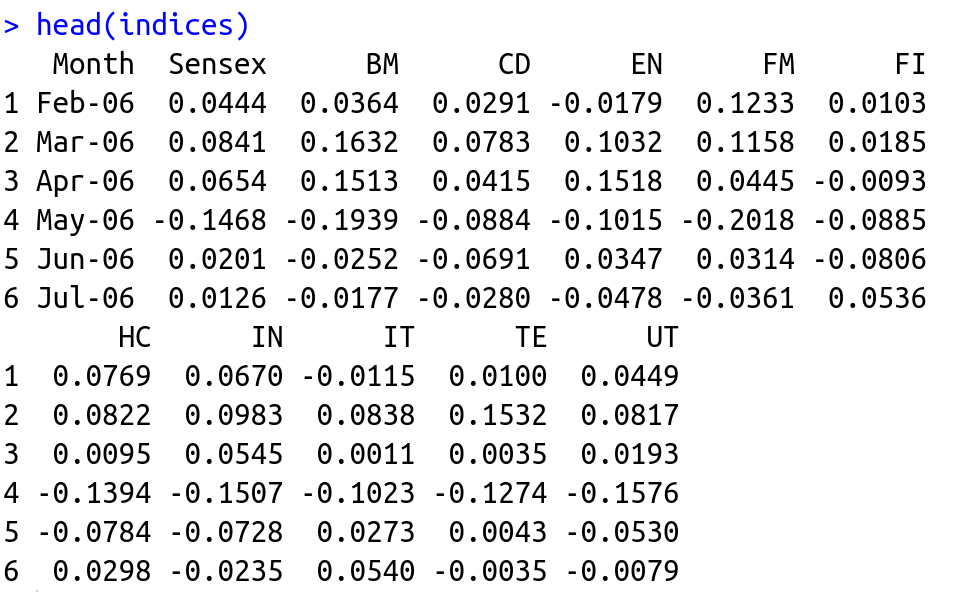
\includegraphics[scale=0.45]{00-D1/images/indices_head.png}
%%%%%%%%%%%%%%%%%%%%%%%%%%%%%%%%%%%%%%%%%%%%%%%%
\newpage 
\subsection*{Exercise 1}

Compute the pairwise Pearson correlation coefficient between the returns of 10 sectors
(BM, CD, EN, FM, FI, HC, IN, IT, TE and UT) rounded to three digits after the decimal point. 
Display the correlation matrix in the output. 


\begin{framed} \begin{verbatim}
# Compute pearson correlation coefficient 

correlation<-cor(indices[,3 : 12], method = "pearson")
correlation<-round(correlation,3) 

correlation 
\end{verbatim}\end{framed} 

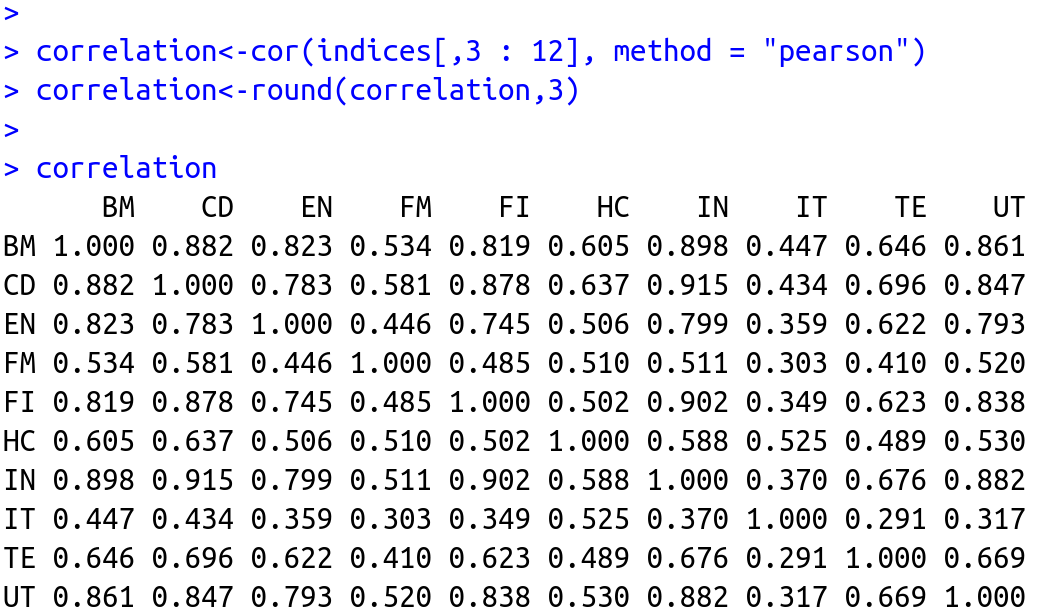
\includegraphics[scale=0.45]{00-D1/images/indices_correlation.png}




%%%%%%%%%%%%%%%%%%%%%%%%%%%%%%%%%%%%%%%%%%%%%%%%
\newpage 
\subsection*{Exercise 2}
\noindent Identify the pair with the highest correlation coefficient and the pair with the least correlation coefficient. 



\begin{framed} \begin{verbatim}
# Pair with Minimum Correlation 

min_cor_location <- which(correlation == min(correlation))

min_cor_location
\end{verbatim}\end{framed} 




\begin{framed} \begin{verbatim}
rownames(correlation)
colnames(correlation)
\end{verbatim}\end{framed} 

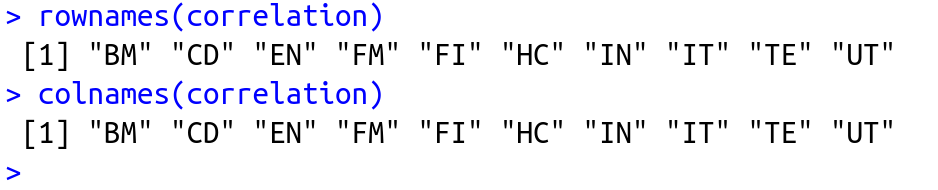
\includegraphics[scale=0.45]{00-D1/images/indices_rownames.png}





\begin{framed} \begin{verbatim}
ceiling(min_cor_location/10)
\end{verbatim}\end{framed} 


<ol class="list-inline">
	<li>8</li>
	<li>9</li>
</ol>




\begin{framed} \begin{verbatim}
min_cor_location %% 10
\end{verbatim}\end{framed} 


<ol class="list-inline">
	<li>9</li>
	<li>8</li>
</ol>




\begin{framed} \begin{verbatim}
ceiling(min_cor_location%%10)
\end{verbatim}\end{framed} 


<ol class="list-inline">
	<li>9</li>
	<li>8</li>
</ol>




\begin{framed} \begin{verbatim}
rownames(correlation)[ceiling(min_cor_location/10)]
\end{verbatim}\end{framed} 


<ol class="list-inline">
	<li>'IT'</li>
	<li>'TE'</li>
</ol>




\begin{framed} \begin{verbatim}
colnames(correlation)[ceiling(min_cor_location%%10)]
\end{verbatim}\end{framed} 


<ol class="list-inline">
	<li>'TE'</li>
	<li>'IT'</li>
</ol>




\begin{framed} \begin{verbatim}

min_cor_pair<-paste(rownames(correlation)[ceiling(min_cor_location/10)],colnames(correlation)[ceiling(min_cor_location%%10)])

min_cor_pair

\end{verbatim}\end{framed} 


\begin{framed} \begin{verbatim}
max_cor_location <- which(correlation == max(correlation[correlation!=1]))

max_cor_pair<-paste(rownames(correlation)[ceiling(max_cor_location/10)]
                    ,colnames(correlation)[ceiling(max_cor_location%%10)])
max_cor_pair

\end{verbatim}\end{framed} 

%%%%%%%%%%%%%%%%%%%%%%%%%%%%%%%%%%%%%%%%%%%%%%%%
\newpage 
\subsection*{Exercise 3}

Perform Principal component analysis on the returns values of the 10 sectors. (4)



\begin{framed} \begin{verbatim}
## Perform a Principal component analysis of the sectoral return values
PCA_corr<-princomp(indices[,3:12])
summary(PCA_corr)
\end{verbatim}\end{framed} 

\begin{verbatim}

    Importance of components:
                              Comp.1      Comp.2     Comp.3     Comp.4      Comp.5
    Standard deviation     0.2106142  0.06763728 0.05825406 0.04631607  0.04255566
    Proportion of Variance 0.7294045  0.07522554 0.05580143 0.03527414  0.02977884
    Cumulative Proportion  0.7294045  0.80463008 0.86043151 0.89570565  0.92548448
    
                               Comp.6     Comp.7     Comp.8      Comp.9     Comp.10
    Standard deviation     0.03735608 0.03326497 0.03093065 0.023803102 0.022500987
    Proportion of Variance 0.02294646 0.01819564 0.01573154 0.009316657 0.008325228
    Cumulative Proportion  0.94843094 0.96662658 0.98235812 0.991674772 1.000000000
    
\end{verbatim}
%%%%%%%%%%%%%%%%%%%%%%%%%%%%%%%%%%%%%%%%%%%55
\newpage 

\newpage Alternatively instead of using \texttt{princomp()}, the student can use \texttt{prcomp()} as
well.


\begin{framed} \begin{verbatim}
PCA_corr_1 <- prcomp(indices[,3:12])

summary(PCA_corr_1)
\end{verbatim}\end{framed} 

\begin{verbatim}

    Importance of components:
                              PC1     PC2     PC3     PC4     PC5     PC6     PC7
    Standard deviation     0.2113 0.06784 0.05843 0.04646 0.04269 0.03747 0.03337
    Proportion of Variance 0.7294 0.07523 0.05580 0.03527 0.02978 0.02295 0.01820
    Cumulative Proportion  0.7294 0.80463 0.86043 0.89571 0.92548 0.94843 0.96663
                               PC8     PC9    PC10
    Standard deviation     0.03103 0.02388 0.02257
    Proportion of Variance 0.01573 0.00932 0.00833
    Cumulative Proportion  0.98236 0.99167 1.00000

\end{verbatim}
%%%%%%%%%%%%%%%%%%%%%%%%%%%%%%%%%%%%%%%%%%%%%%%%
\newpage 
\subsection*{Exercise 4}

\noindent How many principal components have an Eigen value of more than 1? 




\begin{framed} \begin{verbatim}
sum(PCA_corr$sdev^2 )
\end{verbatim}\end{framed} 


0.0608144821839679



\begin{framed} \begin{verbatim}
# Number of PCA components with Eigen value more than 1

sum( PCA_corr$sdev^2 / sum(PCA_corr$sdev^2 ) > (1/10) )

\end{verbatim}\end{framed} 


1


Alternatively


\begin{framed} \begin{verbatim}
sum(PCA_corr_1$sdev^2/sum(PCA_corr_1$sdev^2)>(1/10))
\end{verbatim}\end{framed} 

%%%%%%%%%%%%%%%%%%%%%%%%%%%%%%%%%%%%%%%%%%%%%%%%%%%%%%%%%%%%%%%%%%%%
\newpage 
\subsection*{Exercise 5}

\noindent What is the approximate proportion of total variation explained by the first two principal components? 



\begin{framed} \begin{verbatim}
sum(PCA_corr$sdev^2)
\end{verbatim}\end{framed} 


\begin{framed} \begin{verbatim}
# proportion of total variation explained by the first two principal components
sum(PCA_corr$sdev[1:2]^2)/sum(PCA_corr$sdev^2)
##  0.8046301


\end{verbatim}\end{framed} 


Alternatively

\begin{framed} \begin{verbatim}

sum(hPCA_corr_1$sdev[1:2]^2)/sum(PCA_corr_1$sdev^2)
##  0.8046301
\end{verbatim}\end{framed} 

\newpage

\begin{framed}
\begin{verbatim}
library("FactoMineR")
res.pca <- PCA(decathlon2.active, graph = FALSE)

The output of the function PCA() is a list, including the following components :

print(res.pca)
\end{verbatim}
\end{framed}
%%%%%%%%%%%%%%%%%%%%%%%%%%%%%%%%%%%%%%%%%%%%%%%%
\newpage 
\subsection*{Exercise 6}

Compute the pair wise correlations among the 10 principal components (Round them to 3 digits after the decimal point) and display the results. 

What do you infer about the resulting correlations?



\begin{framed} \begin{verbatim}

# Pairwise correlations of the transformed components

round(cor(PCA_corr$scores),3)
\end{verbatim}\end{framed} 


<table>
<caption>A matrix: 10 x 10 of type dbl</caption>
<thead>
	<tr><th></th><th>Comp.1</th><th>Comp.2</th><th>Comp.3</th><th>Comp.4</th><th>Comp.5</th><th>Comp.6</th><th>Comp.7</th><th>Comp.8</th><th>Comp.9</th><th>Comp.10</th></tr>
</thead>
<tbody>
	<tr><th>Comp.1</th><td>1</td><td>0</td><td>0</td><td>0</td><td>0</td><td>0</td><td>0</td><td>0</td><td>0</td><td>0</td></tr>
	<tr><th>Comp.2</th><td>0</td><td>1</td><td>0</td><td>0</td><td>0</td><td>0</td><td>0</td><td>0</td><td>0</td><td>0</td></tr>
	<tr><th>Comp.3</th><td>0</td><td>0</td><td>1</td><td>0</td><td>0</td><td>0</td><td>0</td><td>0</td><td>0</td><td>0</td></tr>
	<tr><th>Comp.4</th><td>0</td><td>0</td><td>0</td><td>1</td><td>0</td><td>0</td><td>0</td><td>0</td><td>0</td><td>0</td></tr>
	<tr><th>Comp.5</th><td>0</td><td>0</td><td>0</td><td>0</td><td>1</td><td>0</td><td>0</td><td>0</td><td>0</td><td>0</td></tr>
	<tr><th>Comp.6</th><td>0</td><td>0</td><td>0</td><td>0</td><td>0</td><td>1</td><td>0</td><td>0</td><td>0</td><td>0</td></tr>
	<tr><th>Comp.7</th><td>0</td><td>0</td><td>0</td><td>0</td><td>0</td><td>0</td><td>1</td><td>0</td><td>0</td><td>0</td></tr>
	<tr><th>Comp.8</th><td>0</td><td>0</td><td>0</td><td>0</td><td>0</td><td>0</td><td>0</td><td>1</td><td>0</td><td>0</td></tr>
	<tr><th>Comp.9</th><td>0</td><td>0</td><td>0</td><td>0</td><td>0</td><td>0</td><td>0</td><td>0</td><td>1</td><td>0</td></tr>
	<tr><th>Comp.10</th><td>0</td><td>0</td><td>0</td><td>0</td><td>0</td><td>0</td><td>0</td><td>0</td><td>0</td><td>1</td></tr>
</tbody>
</table>




OR Alternatively



\begin{framed} \begin{verbatim}


round(cor(PCA_corr_1$x),3)
\end{verbatim}\end{framed} 

%%%%%%%%%%%%%%%%%%%%%%%%%%%%%%%%%%%%%%%%%%%%%%%%
\newpage 
\subsection*{Interpretation}
The pairwise correlation between the components after the PCA is performed should be zero as PCA is a way to deal with highly correlated variables. 

If N variables are highly correlated than they will all load out on the SAME Principal Component (Eigenvector) and they will be uncorrelated with ot
her components (All these components are orthogonal). Hence the correlations will be zero between the components

\end{verbatim}\end{framed} 

## Exercise 7

Using a scree plot comment on the number of significant components in the model.




\begin{framed} \begin{verbatim}
# Scree Plot
screeplot(PCA_corr,type = "l")



\end{verbatim}\end{framed} 


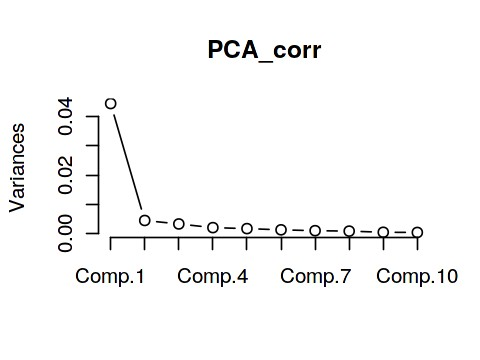
\includegraphics[]{00-D1/images/Indices_Returns_1.jpeg}


%%%%%%%%%%%%%%%%%%%%%%%%%%%%%%%%%%%%%%%%%%%%%%%%%%%%%%%%%%%%%%%%%%%%%%%%%%%%


\begin{framed} \begin{verbatim}
screeplot(PCA_corr_1,type = "l")
\end{verbatim}\end{framed} 


Interpretation: Number of significant components is 1 as the scree plot
almost flattened out after the second component


\end{document}